\documentclass[onepage, 12pt]{beamer}
\mode<presentation>{
	\setbeamercovered{transparent}
	%\beamertemplatenavigationsymbolsempty
	\setbeamertemplate{footline}[frame number]
% 	\usefonttheme{professionalfonts}
}


% https://tex.stackexchange.com/questions/446063/change-background-colour-to-black-and-text-to-white
\usecolortheme{owl}

% https://tex.stackexchange.com/questions/34166/understanding-minipages-aligning-at-top
\usepackage{adjustbox}

% https://tex.stackexchange.com/questions/124256/how-do-i-get-numbered-entries-in-a-beamer-bibliography
\setbeamertemplate{bibliography item}{\insertbiblabel}

% https://tex.stackexchange.com/questions/49048/how-to-cite-one-bibentry-in-full-length-in-the-body-text
\usepackage{bibentry}
\bibliographystyle{plain}
\nobibliography*
%
% https://tex.stackexchange.com/questions/163827/wrong-vertical-spaces-using-bibentry-within-beamer/163842
\def\mybeamernewblock{%
  \usebeamercolor[fg]{bibliography entry author}%
  \usebeamerfont{bibliography entry author}%
  \usebeamertemplate{bibliography entry author}%
  \def\newblock{%
    \usebeamercolor[fg]{bibliography entry title}%
    \usebeamerfont{bibliography entry title}%
    \usebeamertemplate{bibliography entry title}%
    \def\newblock{%
      \usebeamercolor[fg]{bibliography entry location}%
      \usebeamerfont{bibliography entry location}%
      \usebeamertemplate{bibliography entry location}%
      \def\newblock{%
        \usebeamercolor[fg]{bibliography entry note}%
        \usebeamerfont{bibliography entry note}%
        \usebeamertemplate{bibliography entry note}}}}%
  \leavevmode
}
\newenvironment{references}{\begin{itemize}\let\newblock\mybeamernewblock}{\end{itemize}}


\setbeamersize{text margin left=10pt, text margin right=10pt}
\setbeamertemplate{itemize items}[circle]

\beamertemplatenavigationsymbolsempty

% http://tex.stackexchange.com/questions/8680/how-can-i-insert-a-newline-in-a-framebox
%\usepackage{minibox}
%\usepackage{framed}
%\usepackage[usestackEOL]{stackengine}

% https://tex.stackexchange.com/questions/433450/how-to-frame-any-environment-like-minipage-and-others
\usepackage{framed}

% % https://tex.stackexchange.com/questions/91124/itemize-removing-natural-indent
% \usepackage{enumitem}

% % http://tex.stackexchange.com/questions/167000/annotating-tables-with-tikz-adding-arrows
% \usepackage{color, colortbl}
\usepackage{tikz}
\tikzstyle{every picture}+=[remember picture]
%\usetikzlibrary{tikzmark, positioning, fit, shapes.misc}

%% http://tex.stackexchange.com/questions/91124/itemize-removing-natural-indent
%\usepackage{enumitem}

%% http://tex.stackexchange.com/questions/41408/a-five-level-deep-list
%\usepackage{enumitem}
%\setlistdepth{9}

% https://tex.stackexchange.com/questions/20792/how-to-superimpose-latex-on-a-picture
\usepackage{overpic}

% % http://tex.stackexchange.com/questions/32661/how-to-locate-figures-with-x-y-specified-location-in-a-presentation
% \usepackage[absolute,overlay]{textpos} % absolute positioning of stuff
% \setlength{\TPHorizModule}{1mm}
% \setlength{\TPVertModule}{1mm}

\usepackage{graphicx}
\graphicspath{{../img/}}
\AtBeginDocument{\DeclareGraphicsExtensions{.eps, .png, .gif, .pdf, .jpg}}

\usepackage[makeroom]{cancel}

\usepackage[english]{babel}
\usepackage[T1]{fontenc}
\usepackage{times}

% \usepackage{amssymb}
% \usepackage{nicefrac}
% \usepackage{bbm}
% \usepackage{esint}
% \usepackage{sidecap}

\usepackage{hyperref}
% \hypersetup{pdfpagemode=FullScreen}

\newcommand{\HIDE}[1]{}

\newcommand{\skipline}{{\ }\\}

\author{RA}
\subject{Talks}

\newcommand{\CITE}[1]{{\footnotesize[#1]}}

% \input{definitions}

\providecommand{\DIV}{\mathop{\text{div}}}
\providecommand{\GRAD}{\mathop{\text{grad}}}

\providecommand{\IE}{\mathbb{E}}
\providecommand{\IP}{\mathbb{P}}
\providecommand{\IR}{\mathbb{R}}
\providecommand{\IZ}{\mathbb{Z}}

\providecommand{\duality}[2]{\langle #1 \rangle_{#2}}
\providecommand{\norm}[2]{\| #1 \|_{#2}}
\providecommand{\seminorm}[2]{| #1 |_{#2}}
\providecommand{\VERT}{\ensuremath{| \! | \! |}}
\newcommand{\tnorm}[2]{\VERT{#1}\VERT_{{#2}}}

\newcommand{\cA}{\mathcal{A}}
\newcommand{\cB}{\mathcal{B}}
\newcommand{\cL}{\mathcal{L}}
\newcommand{\cN}{\mathcal{N}}
\newcommand{\cT}{\mathcal{T}}
\newcommand{\cX}{\mathcal{X}}
\newcommand{\cY}{\mathcal{Y}}

\providecommand{\Abf}{\mathbf{A}}
\providecommand{\Bbf}{\mathbf{B}}
\providecommand{\Dbf}{\mathbf{D}}
\providecommand{\Ibf}{\mathbf{I}}
\providecommand{\Jbf}{\mathbf{J}}
\providecommand{\Fbf}{\mathbf{F}}
\providecommand{\Hbf}{\mathbf{H}}
\providecommand{\Mbf}{\mathbf{M}}
\providecommand{\Tbf}{\mathbf{T}}
\providecommand{\Pbf}{\mathbf{P}}
\providecommand{\Vbf}{\mathbf{V}}
\providecommand{\pbf}{\mathbf{p}}
\providecommand{\ubf}{\mathbf{u}}
\providecommand{\vbf}{\mathbf{v}}
\providecommand{\wbf}{\mathbf{w}}
\providecommand{\ybf}{\mathbf{y}}
\providecommand{\zbf}{\mathbf{z}}

\renewcommand{\vec}[1]{\mathbf{#1}}

\newcommand{\from}{\colon}

\providecommand{\T}{\mathsf{T}}

\renewcommand{\hat}[1]{\widehat{#1}}
\renewcommand{\tilde}[1]{\widetilde{#1}}

\newcommand{\rd}{\,\mathrm{d}}

\newcommand{\TEXT}[1]{\quad\text{#1}\quad}

% http://tex.stackexchange.com/questions/211518/beamer-vfill-and-itemize
\def\Bottom#1{\vskip 0pt plus 1filll #1}
\def\BottomRight#1{\Bottom{\hfill #1}}

% CODE LISTING
\usepackage{color}
\definecolor{DarkBlue}{rgb}{0,0,0.4}
\definecolor{DarkRed}{rgb}{0.3,0,0}
\definecolor{DarkGreen}{rgb}{0,0.3,0}
\usepackage{listings}
\lstset{%
	language=Python,
	basicstyle=\bf\ttfamily\footnotesize,
	keywordstyle=\color{DarkBlue},
	numbers=left, numberstyle=\footnotesize, numbersep=4pt,
	commentstyle={\color{DarkGreen}},
% 	backgroundcolor=\color{white},
	showspaces=false, showstringspaces=false, showtabs=false,
	frame=none,
	tabsize=4,
	breaklines=true, breakatwhitespace=false,
	emphstyle={[1]\color{blue}},
	emphstyle={[2]\color{DarkGreen}},
	%morekeywords={parfor,true,false},
	xleftmargin=8pt,
	numbers=none
}


%%%%%%%%%%%%%%%%%%%%%%%%%%%%%%%%%%%%%%%%%%%%%%%%%%%%%%%%%%%%%%%%%%%%%%%%%%%%%%%%
%%
%%%%%%%%%%%%%%%%%%%%%%%%%%%%%%%%%%%%%%%%%%%%%%%%%%%%%%%%%%%%%%%%%%%%%%%%%%%%%%%%

\usepackage{ifthen}

\newcommand{\REDBOX}[1]{
	\setlength{\fboxrule}{1pt}
	\fcolorbox{red}{SeeMeBarely}{$\displaystyle
		#1
	$}
}

\definecolor{SeeMeBarely}{RGB}{230,230,230}
\definecolor{Purple}{RGB}{128,0,128}
\definecolor{DeepPurple}{RGB}{32,0,96}
\newcommand{\ra}[1]{{\color{blue}{#1}}}
\newcommand{\cred}[1]{{\color{red}{#1}}}
\newcommand{\cblu}[1]{{\color{blue}{#1}}}
\newcommand{\cpur}[1]{{\color{Purple}{#1}}}

\DeclareMathOperator*{\argmin}{arg\,min}

\newcommand{\ItemComment}[1]{\hfill{\scriptsize(#1)\normalsize}}


% http://www.webnots.com/vibgyor-rainbow-color-codes/
\definecolor{a}{RGB}{148, 0, 211}
\definecolor{b}{RGB}{75, 0, 130}
\definecolor{c}{RGB}{0, 0, 255}
\definecolor{d}{RGB}{0, 160, 0}
\definecolor{e}{RGB}{200, 200, 0}
\definecolor{f}{RGB}{255, 127, 0}
\definecolor{g}{RGB}{255, 0, 0}
%
\definecolor{z}{RGB}{0, 0, 0}
\definecolor{w}{RGB}{255, 255, 255}

% % http://tex.stackexchange.com/questions/17611/how-does-one-type-chinese-in-latex
% \usepackage{CJKutf8}
% \AtBeginDvi{\input{zhwinfonts}}
% %
% \newcommand{\REN}{\begin{CJK*}{UTF8}{gbsn}人\end{CJK*}}
% \newcommand{\ren}[1]{{\color{#1}\REN}}



%%%%%%%%%%%%%%%%%%%%%%%%%%%%%%%%%%%%%%%%%%%%%%%%%%%%%%%%%%%%%%%%%%%%%%%%%%%%%%%%
\begin{document}
%%%%%%%%%%%%%%%%%%%%%%%%%%%%%%%%%%%%%%%%%%%%%%%%%%%%%%%%%%%%%%%%%%%%%%%%%%%%%%%%
%%%%%%%%%%%%%%%%%%%%%%%%%%%%%%%%%%%%%%%%%%%%%%%%%%%%%%%%%%%%%%%%%%%%%%%%%%%%%%%%


\begin{frame}[plain,t]
	\begin{center}
        \vspace{1cm}
		%\small
		%
		Abject mismatch tester gets us
		\\
		{\small\color{gray} Masterclass -- session I}
		%
% 		\\[1\baselineskip]
% 		\small
% 		RA
% 		\\[1\baselineskip]
% 		\footnotesize
% 		\EMAIL

		\vspace{1cm}

		%

	\end{center}

	\Bottom{
		\scriptsize
		R.A.
		\hfill
		BSM, Feb 6, 2020
		\\ {\ }
	}
\end{frame}


%%%%%%%%%%%%%%%%%%%%%%%%%%%%%%%%%%%%%%%%%%%%%%%%%%%%%%%%%%%%%%%%%%%%%%%%%%%%


\begin{frame}[t]{The GRE math subject test}{}
    \begin{itemize}
    \item
        The go-to URL: \href{https://www.ets.org/gre/subject/}{\tt https://www.{\color{blue}ets.org}/gre/subject/}
    
        {\only<1>{
            \begin{quote}
                In general, the questions are intended not only to test recall of information but also to assess the \textbf{understanding} of fundamental concepts and the \textbf{ability to apply} those concepts in various situations.
            \end{quote}
        }}
        
        {\only<1>{%
            Read the FAQ!
%             --
%             \url{https://www.ets.org/gre/subject/faq}
        }}
    \item<2->
        About $2\frac12$ min per question%
        {\only<2>{ (about 66 questions, under 3h)}}.
    \item<3->
        \#2/HB pencil + eraser.
        
        {\only<3>{
            No notes, calculator, \textbf<3>{or extra scratch paper}, etc.
        }}
    \item<4->
        {\color{green}Correct answer: $+1$ point},
        {\color{red}wrong answer: no deduction}.
        
        {\only<4>{%
            \small
            {\ }
            
            From {\tt [go-to URL]}\href{https://www.ets.org/gre/subject/prepare/strategy/}{\tt /prepare/strategy/}:
            
            \begin{quote}
                \color{red}
                Nothing is subtracted [..] if you answer a question incorrectly.
            \end{quote}
            
        }}%
        
        {\only<4>{%
            \small
            \color{gray}
            
            Also, It matters not if you're the only one
            to solve problem X.
        }}%
    \item<5->
        {\only<5->{%
            \emph{Raw score} (\#points) normalized to 
            \emph{scaled score} (200--990).
        }}
    \item<6->
        Typical undergrad material covered.
        
        {\only<6>{
        
            {\ }
        
            \begin{minipage}{0.25\textwidth}
                \Large
                \begin{framed}
                    Calculus \\
                    Diff Eq
                \end{framed}
            \end{minipage}
            %
            \begin{minipage}{0.3\textwidth}
                \begin{framed} 
                    Algebra, trigo \\
                    Linear alg \\ 
                    Abstract alg \\ 
                    Number theory
                \end{framed}
            \end{minipage}
            %
            \begin{minipage}{0.3\textwidth}
                \footnotesize
                \begin{framed}
                    Set theory \\
                    Proba \& stats \\
                    Combinatorics \\
                    Real analysis \\
                    Topology \\
                    Complex variables
                \end{framed}
            \end{minipage}

        }}
    \item<7->
        Good resource: \href{http://rambotutoring.com/math-gre/}{\tt http://{\color{blue}rambo}tutoring.com/}
            
        {\only<7>{
            I'll be using problems from there \& ``The Princeton review''.
        }}
    \item<8->
        Registration (non-US): 
        \textbf{Feb 21} (regular) -- \textbf{Feb 28} (late).
        
        {\only<8>{ 
            {\ }
            
            ...for the next slot Sat, \textbf{Apr 4, 2020}.
        }}
    \item<9->
        {\only<9>{
            Test run.
        }}
    \end{itemize}
    
    \vspace{-10cm}
\end{frame}


%%%


% \begin{frame}[t]{What is a masterclass?}{}
%     \begin{center}
%         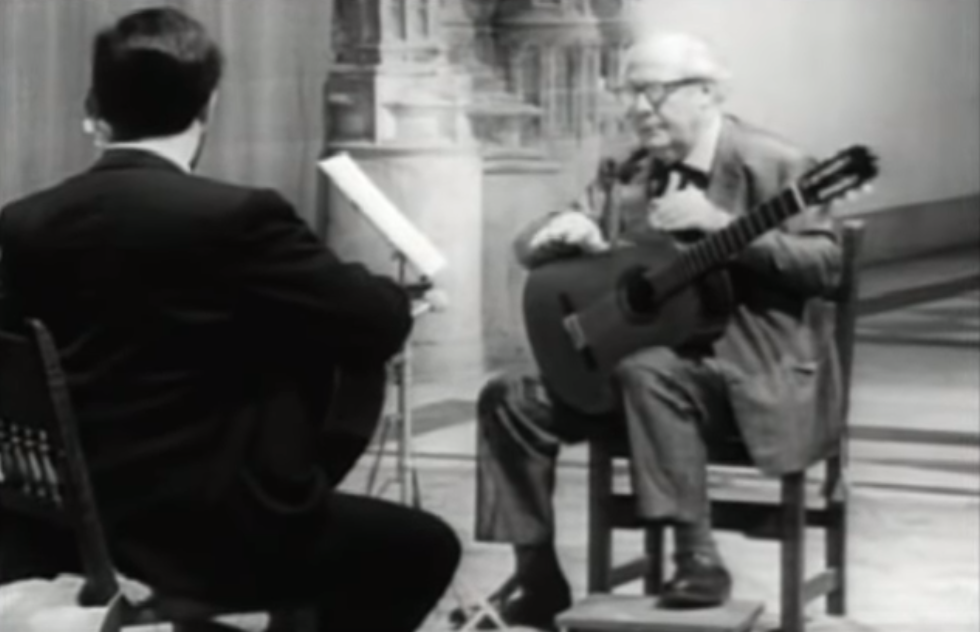
\includegraphics[width=0.7\textwidth]{../../ORIGINALS/lMhqqEfiO3Q}
%         
%         {%
%             O.~Ghiglia with A.~Segovia (1965)
%             
%             \small\url{http://bit.do/segovia}
%         }
%     \end{center}
% \end{frame}


%%%


\begin{frame}[t]{\color{gray} Warm-up}{}
    \begin{align*}
        \int_0^1
        \sqrt{
            e^{2x} + e^{-2x} + 2
        } \, dx
    \end{align*}
\end{frame}


%%%


\begin{frame}[t]{\color{gray} Warm-up}{}
    \begin{align*}
        1 - \frac13 + \frac15 - \frac17 + \ldots
    \end{align*}
\end{frame}



%%%


\begin{frame}[t]{\color{gray} Warm-up}{}
    For how many values of $k \in \IR$ 
    does the system of equations
    \begin{align*}
        k x + y + z & = \only<1>{1} \only<2>{k} \\
        x + k y + z & = k \\
        x + y + k z & = k^2
    \end{align*}
    have no solutions?
\end{frame}


%%%


\begin{frame}[t]{\color{gray} Warm-up}{}
    Let $B \subset \IR^2$.
	%
	Then:
	%
	\begin{quote}
		\normalfont
		$B$ compact.
		
		{\only<1>{$\Rightarrow$}}
		{\only<2>{$\Leftarrow$}}
		
		Every continuous $f \from B \to \IR$ is bounded.
	\end{quote}
\end{frame}

%%%


\begin{frame}[t]{\color{gray} Warm-up}{}
    Let $p \neq q$ be primes.
    %
    {\only<1>{%
        How many abelian groups of order $p^2 q^4$?
    }}%
    %
    {\only<2>{%
        Which of
        $\{ p, p + q, p q, p^q, q^p \}$
        can coexist in a proper subgroup of $(\IZ, +)$?
    }}%
\end{frame}

   



%%%%%%%%%%%%%%%%%%%%%%%%%%%%%%%%%%%%%%%%%%%%%%%%%%%%%%%%%%%%%%%%%%%%%%%%%%%%%%%%%
%\section{Extra}
%%%%%%%%%%%%%%%%%%%%%%%%%%%%%%%%%%%%%%%%%%%%%%%%%%%%%%%%%%%%%%%%%%%%%%%%%%%%%%%%%
%
%
\newcounter{finalframe}
\setcounter{finalframe}{\value{framenumber}}
% Backup frames follow
%
%
% \begin{frame}
% 	Appendix
% \end{frame}
%
%%
%
%\begin{frame}
%	%
%\end{frame}
%
%
% FINAL SLIDE
\setbeamercolor{background canvas}{bg=black}
\begin{frame}[plain,b]
	\hfill
	\tiny
	\color{gray}
	this slide is intentionally left blank
\end{frame}
\setbeamercolor{background canvas}{bg=white}


%%%%%%%%%%%%%%%%%%%%%%%%%%%%%%%%%%%%%%%%%%%%%%%%%%%%%%%%%%%%%%%%%%%%%%%%%%%%%%%%%
%\section{Bibliography}
%%%%%%%%%%%%%%%%%%%%%%%%%%%%%%%%%%%%%%%%%%%%%%%%%%%%%%%%%%%%%%%%%%%%%%%%%%%%%%%%%

% {
% \tiny
% \bibliography{../../../r/refs}
% }


%%%%%%%%%%%%%%%%%%%%%%%%%%%%%%%%%%%%%%%%%%%%%%%%%%%%%%%%%%%%%%%%%%%%%%%%%%%%%%%%
\setcounter{framenumber}{\value{finalframe}}
\end{document}
%%%%%%%%%%%%%%%%%%%%%%%%%%%%%%%%%%%%%%%%%%%%%%%%%%%%%%%%%%%%%%%%%%%%%%%%%%%%%%%%
%%%%%%%%%%%%%%%%%%%%%%%%%%%%%%%%%%%%%%%%%%%%%%%%%%%%%%%%%%%%%%%%%%%%%%%%%%%%%%%%

